\documentclass[a4paper]{article} 
\usepackage{graphicx} 
\usepackage[ngerman]{babel} 
\usepackage[ansinew]{inputenc} 
\usepackage[T1]{fontenc} 
\usepackage{tgpagella} 
\usepackage{geometry} 
\usepackage{color} 
\usepackage{microtype} 
\usepackage{minted}
\usepackage{caption}
\usepackage[headsepline,footsepline]{scrpage2}
\usepackage{textcomp}
\usepackage{pdfpages}
\usepackage{mdframed}



\makeatletter
\renewcommand\minted@pygmentize[2][\jobname.pyg]{
  \def\minted@cmd{pygmentize -l #2 -f latex -F tokenmerge
    \minted@opt{gobble} \minted@opt{texcl} \minted@opt{mathescape}
    \minted@opt{startinline} \minted@opt{funcnamehighlighting}
    \minted@opt{linenos} -P "verboptions=\minted@opt{extra}"
    -O encoding=UTF-8,outencoding=iso-8859-1 -o \jobname.out.pyg #1}
  \immediate\write18{\minted@cmd}
  % For debugging, uncomment:
  %\immediate\typeout{\minted@cmd}
  \ifthenelse{\equal{\minted@opt@bgcolor}{}}
   {}
   {\begin{minted@colorbg}{\minted@opt@bgcolor}}
  \input{\jobname.out.pyg}
  \ifthenelse{\equal{\minted@opt@bgcolor}{}}
   {}
   {\end{minted@colorbg}}
  \DeleteFile{\jobname.out.pyg}}
\makeatother


\title{Dokumentation - 6 Übung}
\author{Roman Lumetsberger}
\date{\today}

\newmintedfile[ccode]{cpp}{
               linenos,
               numbersep=5pt,
               frame=lines,
               framesep=2mm
}

\newmintedfile[javacode]{java}{
               linenos,
               numbersep=5pt,
               frame=lines,
               tabsize=2,
               framesep=2mm,
}
\newmintedfile[csscode]{css}{
               linenos,
               numbersep=5pt,
               frame=lines,
               tabsize=2,
               framesep=2mm,
}
\newmintedfile[sqlcode]{sql}{
               linenos,
               numbersep=5pt,
               frame=lines,
               tabsize=2,
               framesep=2mm,
}
\captionsetup{
  font=footnotesize,
  justification=raggedright,
  singlelinecheck=false
}


\newcommand{\srcDir}{../Beispiel/src/at/lumetsnet/caas/}
\newcommand{\testDir}{../Beispiel/test/at/lumetsnet/caas/test/}

\definecolor{lineColor}{RGB}{151,0,0}
\pagestyle{scrheadings}
\clearscrheadfoot
\begin{document}
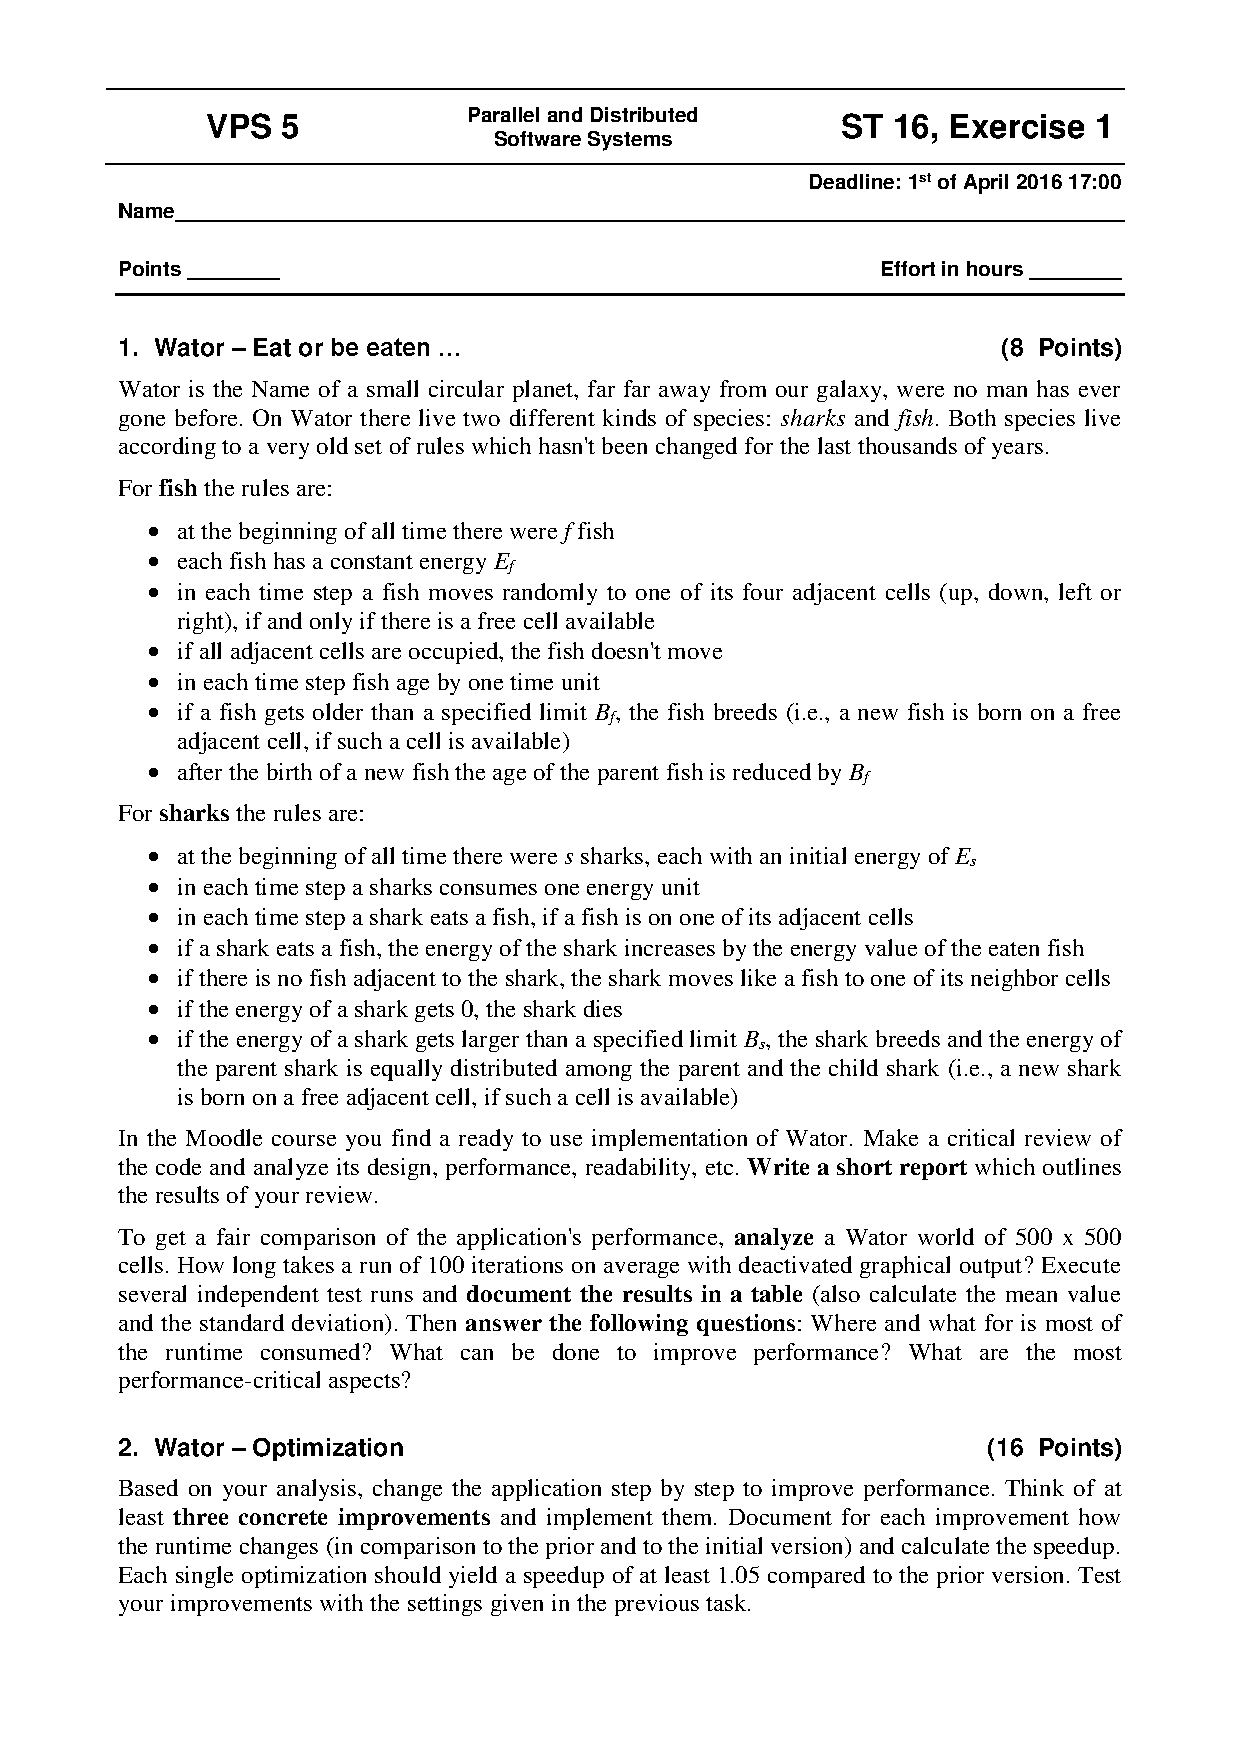
\includepdf[pages=-]{angabe.pdf}

\ihead{VPS SS 2016 - �bung 01}
\ifoot{Roman Lumetsberger}
\cfoot{1310307026}
\ofoot{Seite \pagemark}

\section{1. Wator � Eat or be eaten}
\subsection{Analyse}
Der Sourcecode ist grunds�tzlich gut dokumentiert und auch lesbar. 
Die Architektur der Anwendung loose gekoppelt und nachvollziehbar. Zur Implementierung gibt es zu erw�hnen, dass in der selben Methode oft auf die gleichen Feldelemente zugegriffen wird. Hier w�re es vielleicht
besser, wenn der Wert einmal zwischengespeichert werden w�rde, da sonst bei jedem Zugriff Laufzeit�berpr�fungen durchgef�hrt werden. 
Weiters f�llt auf, dass sehr viele Objekte der Klasse \texttt{Point} angelegt werden.
Zur Methode \texttt{GetNeighbors} gibt es zu erw�hnen, dass hier f�r alle vier Richtungen eigentlich der selbe Code verwendet wird und dieser vielleicht besser in eine Methode ausgelagert werden k�nnte (bringt 
warscheinlich keine Performancesteigerung aber der Code w�re besser lesbar).

\subsection{Where and what for is most of the runtime consumed?}
 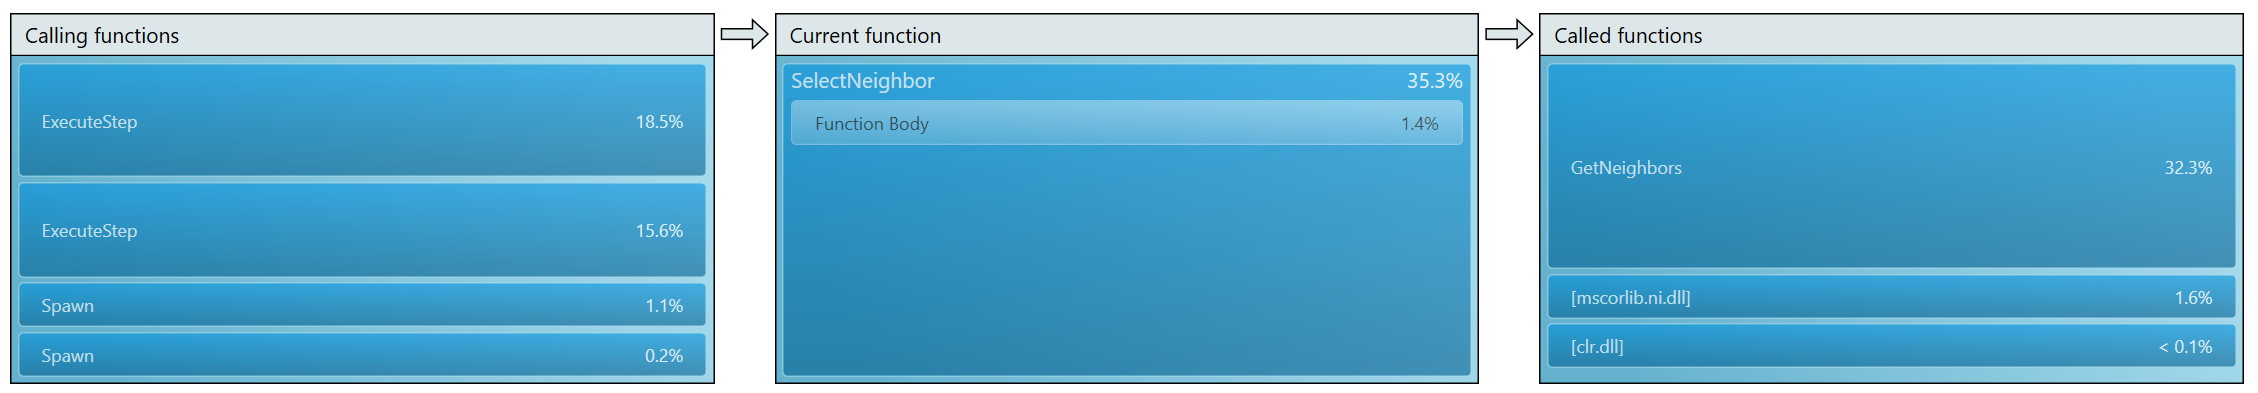
\includegraphics[width=400px]{images/profiling.png}


 Grunds�tzlich wird die meiste CPU-Zeit in der Methode \texttt{ExecuteStep} und in weiterer Folge dann in \texttt{GetNeighbors} verbraucht.
 Diese Methode ist f�r das Suchen der Nachbarn eines Feldes zust�ndig und wird daher sehr oft aufgerufen.
 Die Analsyse der Methode zeigt, dass sehr viele \texttt{Point} Objekte angelegt und dann sogar nochmals kopiert werden. Dadurch wird sehr viel CPU-Zeit verbraucht.

 Die Methode \texttt{RandomizeMatrix} ist eine weitere Methode die sehr viel CPU-Zeit ben�tigt. Diese ist f�r das Mischen der Durchlauf-Matrix zust�ndig.

\subsection{Performance}
Ohne Optimierungen liefert das Programm folgende Werte

\includegraphics[width=300px]{images/OriginalVersion.png}

\subsection{What can be done to improve performance?}
\begin{itemize}
	\item Umgang mit den Koordinaten in der Methode \texttt{GetNeighbors} optimieren, damit nicht mehr so viele Objekte angelegt werden m�ssen.
		\subitem Verwenden eines statischen Arrays.
		\subitem Kopieren des Arrays am Ende der Methode vermeiden.
	\item Umstellen der zweidimensionalen Felder auf eindimensionales Felder.
	\item �ndern \texttt{Moved} Eigenschaft um die zus�tzliche Schleife �ber alle Elemente zu sparen.
		\subitem Eine M�glichkeit w�re hier die Iterationsnummer zu verwenden. 
\end{itemize}
  
\section{2. Wator � Optimization }

\subsection{Version 1}
F�r diese Optimierung wurde versucht die Anzahl der ben�tigten \texttt{Point} Objekte zu verringern indem die Methode \texttt{GetNeighbors} folgenderma�en ge�ndert wurde.
Die lokale Variable \texttt{neighbors} wurde als private Datenkomponente angelgt und wird so f�r jeden Aufruf wiederverwendet und braucht nicht neu angelegt werden.

Weiters wurde die Logik der zuf�lligen Auswahl einer Richtung direkt in die Methode \texttt{GetNeighbors} verlagert, damit braucht am Ende das Array nicht kopiert werden, sonder 
es wird direkt der Punkt zur�ckgegeben.

Zur besseren Lesbarkeit des Quellcodes wurde die Pr�fung, ob ein Nachbarelement g�ltig ist in eine eigene Methode \texttt{CheckNeighbor} ausgelagert.

\subsection{Performance}
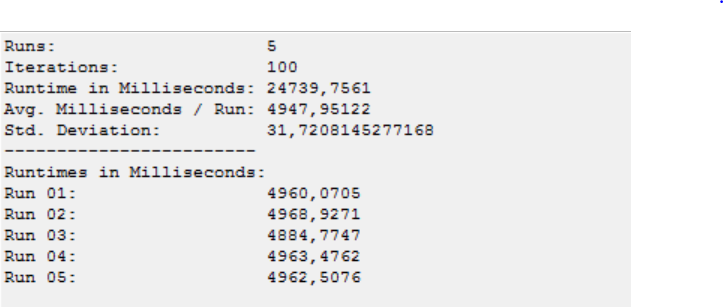
\includegraphics[width=300px]{images/Version1.png}\linebreak
Speedup und �nderung zu vorherigen Version siehe Zusammenfassung.

\subsubsection{Code�nderungen}
\begin{minted}[
frame=lines,
fontsize=\footnotesize,
]{csharp}
/// <summary>
/// Neighbors static data array which is reused
/// </summary>
private readonly Point[] neighbors = new Point[4];
\end{minted}

\begin{minted}[
frame=lines,
fontsize=\footnotesize,
tabsize=2
]{csharp}
 /// <summary>
/// Neighbors static data array which is reused
/// </summary>
private readonly Point[] neighbors = new Point[4];

// find all neighbouring cells of the given position that contain an animal of the given type
public Point SelectNeighbor(Type type, Point position)
{
		int neighborIndex;
		int i, j;

		// counter for the number of cells of the correct type
		neighborIndex = 0;
		// look up
		i = position.X;
		j = (position.Y + Height - 1) % Height;
		if (CheckNeighbor(type, i,j ))
		{
				neighbors[neighborIndex].X = i;
				neighbors[neighborIndex].Y = j;
				neighborIndex++;
		}

		i = (position.X + 1) % Width;
		j = position.Y;
		if (CheckNeighbor(type,i, j))
		{
				neighbors[neighborIndex].X = i;
				neighbors[neighborIndex].Y = j;
				neighborIndex++;
		}

		// look down
		i = position.X;
		j = (position.Y + 1) % Height;
		if (CheckNeighbor(type, i, j))
		{
				neighbors[neighborIndex].X = i;
				neighbors[neighborIndex].Y = j;
				neighborIndex++;
		}

		// look left
		i = (position.X + Width - 1) % Width;
		j = position.Y;
		if (CheckNeighbor(type, i, j))
		{
				neighbors[neighborIndex].X = i;
				neighbors[neighborIndex].Y = j;
				neighborIndex++;
		}

		if (neighborIndex > 1)
		{
				// if more than one cell has been found => return a randomly selected cell
				return neighbors[random.Next(neighborIndex)];
		}
		else if (neighborIndex == 1)
		{
				// if only a single cell contains an animal of the given type we can save the call to random
				return neighbors[0];
		}
		else
		{
				// return a point with negative coordinates to indicate
				// that no neighbouring cell has found
				// return value must be checked by the caller
				return new Point(-1, -1);
		}
}
/// <summary>
/// Checks if a neighbor is from the given type
/// </summary>
private bool CheckNeighbor(Type type, int xCoord, int yCoord)
{
		var value = Grid[xCoord, yCoord];
		if ((type == null) && (value  == null))
		{
				return true;
		}
		else if ((type != null) && (type.IsInstanceOfType(value)))
		{
				if ((value != null) && (!value.Moved))
				{
						return true;
				}
		}
		return false;
}
\end{minted}
	

\subsection{Version 2}
In dieser Version wurde das zweidimensionale Feld \texttt{randomMatrix} in ein eindimensionales Feld ge�ndert. 
Damit ist k�nnen die Methoden \texttt{GenerateRandomMatrix} und \texttt{RandomizeMatrix} wesentlich einfacher implmentiert werden. Weiters ben�tigt der die Methode \texttt{RandomizeMatrix} nur mehr einen
Aufruf von \texttt{random.Next}.

\subsection{Performance}
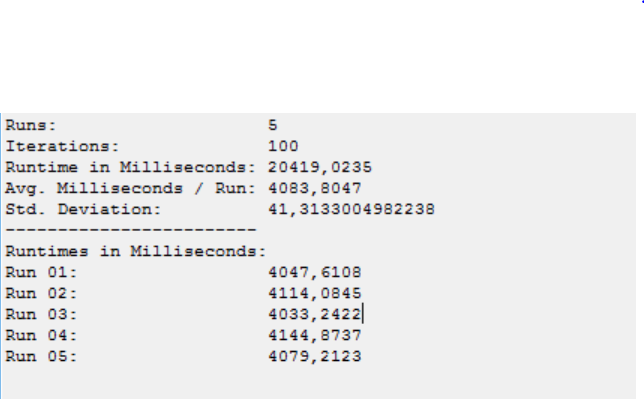
\includegraphics[width=300px]{images/Version2.png}\linebreak
Speedup und �nderung zu vorherigen Version siehe Zusammenfassung.

\subsubsection{Code�nderungen}
\begin{minted}[
frame=lines,
tabsize=2,
fontsize=\footnotesize,
]{csharp}
private int[] randomMatrix;


// create a 2D array containing all numbers in the range 0 .. width * height
// the numbers are shuffled to create a random ordering
private int[] GenerateRandomMatrix(int width, int height)
{ 
		int[] matrix = new int[width * height];

		for (int i = 0; i < matrix.Length; i++)
		{
			 matrix[i]=i;
		}
		// shuffle matrix
		RandomizeMatrix(matrix);
		return matrix;
}

// shuffle the values of the 2D array in a random fashion
private void RandomizeMatrix(int[] matrix)
{
		//Knuth shuffle for arrays 
		//https://www.rosettacode.org/wiki/Knuth_shuffle#C.23
		for (int i = 0; i < matrix.Length; i++)
		{
				int j = random.Next(i, matrix.Length); // Don't select from the entire array on subsequent loops
				int temp = matrix[i];
				matrix[i] = matrix[j];
				matrix[j] = temp;
		}
}

public void ExecuteStep()
{
...
// go over all cells of the random matrix
		int row, col;
		for (int i = 0; i < Width*Height; i++)
		{
				// determine row and col of the grid cell by manipulating the value
				var value = randomMatrix[i];
				col = value % Width;
				row = value / Width;

				// if there is an animal on this cell that has not been moved in this simulation step
				// then we execute it
				if (Grid[col, row] != null && !Grid[col, row].Moved)
						Grid[col, row].ExecuteStep();
				
		}
...
\end{minted}


\subsection{Version 3}
In der dritten Optimierung wurde die Notwendigkeit des zus�tzlichen Schleifendurchlaufs um das \texttt{Commit} auszuf�hren. Dazu wurde eine neue Datenkomponente \texttt{CurrentIteration} eingef�hrt und beim
Property \texttt{Moved} wird dann der Iterationsz�hler verglichen.

\subsection{Performance}
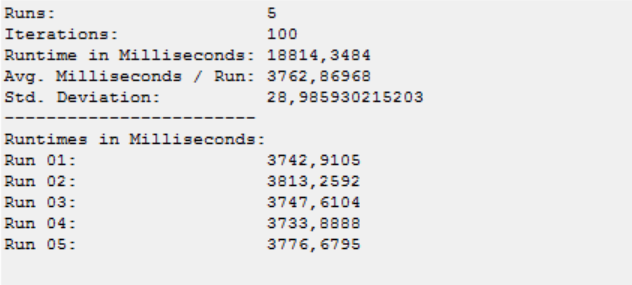
\includegraphics[width=300px]{images/Version3.png}\linebreak
Speedup und �nderung zu vorherigen Version siehe Zusammenfassung.

\subsubsection{Code�nderungen}
\begin{minted}[
frame=lines,
tabsize=2,
fontsize=\footnotesize,
]{csharp}
public abstract class Animal
{
...
	//iteration in which the animal was moved
	private long movedIteration;
	
	// ctor: create a new animal on the specified position of the given world
	public Animal(OriginalWatorWorld world, Point position)
	{
...
			movedIteration = World.CurrentIteration;
...
	}
	
	// move the animal to a given position
	// does not check if the position can be reached by the animal
	protected void Move(Point destination)
	{
		World.Grid[Position.X, Position.Y] = null;
		World.Grid[destination.X, destination.Y] = this;
		Position = destination;
		movedIteration = World.CurrentIteration;
	}


	// boolean flag that indicates wether an animal has moved in the current iteration
	public bool Moved
	{
			get { return movedIteration == World.CurrentIteration; }
	}
	
\end{minted}

\begin{minted}[
frame=lines,
tabsize=2
fontsize=\footnotesize,
]{csharp}
public class OriginalWatorWorld : IWatorWorld
{
	...	
		/// <summary>
		/// Gets the current iteration of the world
		/// </summary>
		public long CurrentIteration { get; private set; }
	
	public void ExecuteStep()
	{
			CurrentIteration++;
			...
			
	}
	...
}
\end{minted}

\section{Zusammenfassung}
% Please add the following required packages to your document preamble:
% \usepackage{booktabs}
\begin{table}[!htbp]

\caption{Ergebnis}
\label{summary}
\begin{tabular}{@{}lllll@{}}
\cmidrule(l){2-5}
                             & Original   & Version 1  & Version 2   & Version 3  \\ \midrule
1 LAUF                       & 6275,0363  & 4960,0705  & 4047,6108   & 3742,9105  \\ \midrule
2 LAUF                       & 6573,7986  & 4968,9271  & 4114,0845   & 3813,2592  \\ \midrule
3 LAUF                       & 6059,9067  & 4884,7747  & 4033,2422   & 3747,6104  \\ \midrule
4 LAUF                       & 5996,6139  & 4963,4762  & 4144,8737   & 3733,8888  \\ \midrule
5 LAUF                       & 6001,7686  & 4962,5076  & 4079,2123   & 3776,6795  \\ \midrule
DURCHSCHNITT                 & 6181,42482 & 4947,95122 & 4083,8047   & 3762,86968 \\ \midrule
STANDARDABWEICHUNG           & 220,870269 & 31,7208145 & 41,3133005  & 28,9859302 \\ \midrule
SPEEDUP ZU VORIGEN VERSION   &           & 1,24726873 & 1,21160329  & 1,0852900  \\ \midrule
SPEEDUP ZUR ORIGINAL VERSION &           & 1,24726873 & 1,513643593 & 1,6427422  \\ \bottomrule
\end{tabular}
\end{table}
\end{document}